%%%%%%%%%%%%%%%%%%%%%%%%%%%%%%%%%%%%%%%%%%%%%%%%%%%%%%%%%%%%%%%%%
%  _____       ______   ____									%
% |_   _|     |  ____|/ ____|  Institute of Embedded Systems	%
%   | |  _ __ | |__  | (___    Wireless Group					%
%   | | | '_ \|  __|  \___ \   Zuercher Hochschule Winterthur	%
%  _| |_| | | | |____ ____) |  (University of Applied Sciences)	%
% |_____|_| |_|______|_____/   8401 Winterthur, Switzerland		%
%																%
%%%%%%%%%%%%%%%%%%%%%%%%%%%%%%%%%%%%%%%%%%%%%%%%%%%%%%%%%%%%%%%%%

\chapter{\textit{testbench}}\label{chap.testen}
Inspiriert vom Konzept des \textit{test driven development} wird stets parallel zur Entwicklung einer \textit{unit} (im folgenden als Block genannt) der \textit{unit-test} entwickelt \cite{Testdriven}.

Nachdem im Voraus die Schnittstellen zwischen den Blocks geklärt sind (\textbf{siehe Kapitel xXX}) wird eine leere Hülle für jeden zu entwickelnden Block erstellt. Die \textit{testbench} geht von Beginn weg vom Ziel, eines funktionstüchtigen \textit{midi interface} aus. Solange ein Block noch nicht fertig entwickelt ist, führend erst partiell korrekt führende Signale an den Ausgang der DUT. Mit jeder zusätzlichen Implementation, wird das Verhalten der Signale korrekter.\\

\begin{figure}[H]
	\centering
	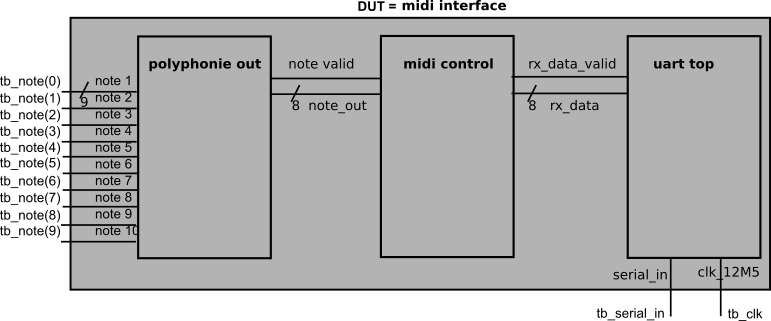
\includegraphics[width=1\textwidth]{images/midi_interface/testbench_midiinterface.png}
	\caption{Blockschaltbild Device under Test}
	\label{fig.testbench}
\end{figure}

Eine Bedingung an die Projektarbeit ist, dass die Tests textbasiert ablaufen sollen (siehe Aufgabenstellung im Anhang \ref{chap.anhang_aufgabenstellung_neu}). Diese zusätzliche Spezifikation wird hier kurz zusammengefasst.

\section{Textbasierte Testbench}\label{sec.testbench}
Die zu testenden Befehle stammen aus der Datei input\_midi.txt. Der Inhalt ist aufgelisten im Anhang \ref{chap.anhang_midi_input}.
\subsection{Struktur der Testserie}
Ausgehend von der MIDI 1.0 Spezifikation, wird die Funktion des \textit{single modes} und des \textit{polyphony modes} getestet. Der Testablauf hängt von dem zu testenden Fall ab: Weil die \textit{data bytes} im \textit{polyphony mode} anders sind, als im \textit{single mode}, baut sich der Test auch anders auf.\\
\subsubsection{Setzen des Testmodus} 
Damit das Programm weiss, nach welchem Aufbau es die Signale senden muss, wird zuerst der Testmode eingestellt. Dies ist das erste Wort jeder Zeile im Testscript.\smallskip
\begin{tabbing}

\textbf{reset} 	 \= 00  \= 00  \=....\\
\textbf{check} \>00	\>00 \>....\\
\textbf{singl} \>  55 \>90 \>....\\
\end{tabbing}

Den Testmodus \textbf{reset} braucht es, da keine manuellen Tests in die \textit{testbench} eingeführt werden. Den Testmodus \textbf{check} beinhaltet die zu erwartenden Ergebniswerte, wenn der vorhin gesetzte Testmode korrekt abläuft.\\
Da das Testmodus Kommando-Wort immer gleich lang sein muss (hier 5 Buchstaben) sind die Wörter grammatikalisch nicht korrekt. Aus polyphony wurde polyp. 

Der Tokenaufbau der zwei Testmodes \textit{single mode} und \textit{polyphony mode }
wird nun genauer erklärt:

\subsubsection{Einzelne Noten testen }
Das Testen einer einzelnen Note ist einfach. Da gemäss Spezifikation zuerst ein \textit{status byte} mit der Meldung Note on (0x90) oder Note off (0x80) kommt. Und dann das \textit{data byte} mit dem Notenwert folgt. Die Geschwindigkeit ist für das An- oder Abstellen der Note nicht relevant und wird deshalb nicht als Befehl eingelesen. Die \textit{testbench} hängt selbständig im single mode nach jeder Note einen Dummy-Geschwindigkeitswert von 0x55 an. \bigskip

\underline{Zeile in der Datei}\\
singl \hspace*{3mm} 55 \hspace*{4mm} 90 \hspace*{12mm}  27 \hspace*{6mm} 80 \hspace*{10mm} 27 \hspace*{6mm} 90 \hspace*{10mm} 05 \hspace*{6mm} 00 \hspace*{12mm} 00\\
check \hspace*{2mm} 00 \hspace*{4mm} 00 \hspace*{12mm}  27 \hspace*{6mm} 00 \hspace*{10mm} 00 \hspace*{6mm} 00 \hspace*{10mm} 05 \hspace*{6mm} 00 \hspace*{12mm} 00\\

\underline{Tokenaufbau}\\
mode	\hspace{2mm} Note \hspace*{2mm} 	Velocity	\hspace*{2mm} Note \hspace*{2mm}  Velocity \hspace*{2mm} 	Note \hspace*{2mm} 	Velocity \hspace*{2mm} 	Note \hspace*{2mm} 	Velocity \hspace*{2mm}  Anzahl Noten an

Die hier abgebildete Sequenz bedeutet: Note 27 anstellen (0x90 ist das status byte für Note an), dann Abstellen der Note 27 und am Schluss Anstellen der Note 05. \\
Überprüft am Schluss der Sequenz die \textit{testbench} den Ausgang des \textit{midi interfaces}, so erscheinen die zwei Notenwerte 27 und 05.

Im Fall der einzelnen Note passt die Tokenstruktur, die sich am schwierigsten Fall, der Polyphonie orientierte, nicht ganz. Im Gegensatz zur Polyphonie muss bei der einzlenen Note VOR dem Notenwert ein status byte kommen. Damit dies in der Tokenstruktur umsetzbar ist, wird zuerst ein Dummy-Wert (55) zum Verwerfen der \textit{testbench} übergeben. Erst dann folgt das \textit{status byte} und dann, analog zur Polyphony-Sturktur folgt die erste Note. Im Nachhinein erscheint mir dieser Aufbau als zu kompliziert und ich würde ein nächstes Mal mehr mode-spezifisch die Datenauswertung gestalten.




\subsubsection{Polyphonie testen }

\underline{Zeile in der Datei}\\
polyp \hspace*{2mm} 71 \hspace*{4mm} 55 \hspace*{12mm}  02 \hspace*{6mm} 55 \hspace*{10mm} 33 \hspace*{6mm} 55 \hspace*{10mm} 08 \hspace*{6mm} 00 \hspace*{12mm} 00\\
check \hspace*{2mm} 71 \hspace*{4mm} 00 \hspace*{12mm}  02 \hspace*{6mm} 00 \hspace*{10mm} 33 \hspace*{6mm} 00 \hspace*{10mm} 00 \hspace*{6mm} 00 \hspace*{12mm} 03\\

\underline{Tokenaufbau}\\
mode	\hspace{2mm} Note \hspace*{2mm} 	Velocity	\hspace*{2mm} Note \hspace*{2mm}  Velocity \hspace*{2mm} 	Note \hspace*{2mm} 	Velocity \hspace*{2mm} 	Note \hspace*{2mm} 	Velocity \hspace*{2mm}  Anzahl Noten an\\

Das bedeutet, dass die \textit{testbench} im Testmodus Polyphonie ist. Und deshalb als erstes das \textit{status byte} der Polyphonie "10100000" (0xA0) senden muss. Danach werden die Token gemäss der Polyphonie-Spezifikation interpretiert: Die \textit{data bytes} wechseln sich ständig mit dem Notenwert und der dazugehörenden Geschwindigkeit ab. Hier in der Testdatei hält die erste Note den Wert 71 und wird gefolgt von irgendeiner Geschwindigkeit (hier Dummy-Wert 55), usw.. Kommt ein Geschwindigkeitswert von 0, so bedeutet dies, dass die Note abgestellt wird.
In der Polyphonie ist das Note An- und Abstellen asynchron. Der Befehl folgt nicht automatisch nach jedem Notenbyte. Aus diesem Grund weiss man nicht indirekt, wie viele Noten zu einem gewissen Zeitpunkt an sind. Aus diesem Grund gibt es den letzten Token: Anzahl Noten an. Dieser sagt der testbench wie viele Noten an sein sollen.
Beim Überprüfen des Ausganges des \textit{midi interfaces} muss nach der ersten Befehlzeile die drei Noten 71, 02 und 33 an sein. Was einer Summe von drei entspricht.







\section{code der testbench}\label{sec.code_testbench}
Im Gegensatz zum hardwarenahen Code der VHDL-Blocks, bei denen arrays und loop explizit vermieden wurden, baute die \textit{testbench} bewusst auf softwarenahe Strukturen auf.

\subsection*{package}
Es ist ein Package für die Konstanten der der \textit{status bytes} und für die Noten-Verarbeitung erstellt.
\smallskip

Die Tokenstruktur wurde wiefolgt implementiert: \\  
\smallskip 

-- define midi\_data\\
type t\_midi\_data is record  \\                    
\hspace*{12mm}        token\_note : std\_logic\_vector(7 downto 0);  \\                  
\hspace*{12mm}        token\_attribut : std\_logic\_vector(7 downto 0);\\
\hspace*{12mm}    end record;\\

\smallskip
type t\_midi\_data\_array is array (0 to 3) of t\_midi\_data;\\

-- define token structure\\
type t\_token\_line is record\\
\hspace*{12mm}        token\_cmd : string(1 to 5);\\
\hspace*{12mm}        t\_midi\_data : t\_midi\_data\_array;\\
\hspace*{12mm}        token\_number : std\_logic\_vector(7 downto 0);\\
\hspace*{12mm}    end record;\\


        
-- array with note structure (input/output)     \\
type t\_note\_array is array (0 to 9) of std\_logic\_vector(8 downto 0);\\

\subsection*{Prozessstruktur}
%Strukturmässig über Allem steht bei der textbasierten \textit{testbench} das Ein- und Auslesen der Dateien. Nach dem Grunsatz in der Software, dass Prozesse möglichst kurz und nur etwas erledigen sollen, begann ich den Prozess zu unterteilen in einen \textit{read file}-Prozess und einen \textit{execute file}-Prozess. Die zwei Prozesse sind über das Signal-Flag s\_read\_input\_finished synchronisiert, das im \textit{execute file}-Prozess mit dem Befehl \textit{wait until} (s_read_input_finished <= '1') umgesetzt ist.\\

Durch das Aufteilen der Prozesse ergab sich auch die Unterscheidung zwischen lokalen Variablen und Signalen.

\section{ergebnisse simulation}\label{sec.ergebnisse_tests}


